\section{Formalization of Buddy Allocation Model}
The formalization of the buddy allocation memory management consists of a model for the necessary data structures to represent the memory, and for the allocation and disposal operations memory management provides. This formalization follows the algorithms for the buddy allocation memory management in Zephyr OS~\cite{}, which applies a quartering split over nodes.

%This approach is more practical because it aims to pursue the efficiency. Since our specification requires a detailed description of the algorithms as well as the complex quartering way to describe, the foreseeable result is that it brings complexity to proofs than those abstract memory models.

To guarantee functional correctness of the formal model we proof a number of properties related to the transformations that the operations carry out over the memory structure. We try to answer the following questions: do the operations pick out the most suitable block from all the available blocks? is the state of the data structures representing the memory correctly set after executing the operations? are free blocks properly merged after a disposal operation? Answering these questions contributes to the construction of a reliable memory system.

\subsection{Memory Model Specification}
The specification begins with the structure of a quad-tree.
\begin{align*}
(set:\ 'a)\ tree = &Leaf\ (L:\ 'a)\ | \\
&Node\ (LL:\ 'a\ tree)\ (LR:\ 'a\ tree)\ (RL:\ 'a\ tree)\ (RR:\ 'a\ tree) \\
&for\ map: tree\_map
\end{align*}
The quad-tree constructed by induction contains two pieces of information: the memory block type (indicated as \emph{ALLOC} and \emph{FREE} respectively); a address tag occupied by a memory block (indicated as \emph{ID}). The mapping function \textbf{tree.set} assists to collect the leaves from a tree. With the help of the block \textbf{type} and the function \textbf{get\_level} in a quad-tree, allocated leaves or free leaves from different levels can be gathered by \textbf{allocsets}, \textbf{freesets} and \textbf{freesets\_level}. All used \emph{ID} labels are in \emph{idset}. To create a new leaf, we have to pick up a new \emph{ID} to this new leaf by the strategy of \emph{SOME p. p} $\notin$ \emph{idset}. Later, we will prove that with this strategy, all leaves have different \emph{ID} labels.

Based on the above structure of a quad-tree, next we specify two operations with the buddy algorithms: \textbf{alloc} and \textbf{free}. For \emph{rsize} (the size of requested memory block) in allocation operation, there is a function that maps it to the level of the quad-tree and returns the most suitable level \emph{rlv}. The concept of \emph{most suitable level} will be proved in the next subsection. For the specification, we only use levels for both memory blocks in the quad-trees and requested memory blocks. And the smaller the level, the larger size the memory block.

\begin{definition} [existence of free blocks in a level] \\
	exists\_freelevel blo\_set lv $\equiv$ $\exists$l. l $\leq$ lv $\wedge$ $\exists$b $\in$ blo\_set. freesets\_level b l $\ne$ $\emptyset$
\end{definition}

\begin{definition} [maximum level of free blocks] \\
	freesets\_maxlevel blo\_set lv $\equiv$ \\
	\phantom{x} \hspace{10pt} THE lmax. lmax $\leq$ lv $\wedge$ \\
	\phantom{x} \hspace{60pt} $\exists$b $\in$ blo\_set. freesets\_level b lmax $\neq$ $\emptyset$ $\wedge$ \\
	\phantom{x} \hspace{60pt} $\forall$l $\leq$ lv. $\exists$b $\in$ blo\_set. freesets\_level b l $\ne$ $\emptyset$ $\longrightarrow$ l $\leq$ lmax
\end{definition}

\begin{definition} [Allocation Operation] \\
	alloc blo\_set rlv $\equiv$ \\
	\phantom{x} \hspace{10pt} if exists\_freelevel blo\_set rlv then \\
	\phantom{x} \hspace{20pt} lmax = freesets\_maxlevel blo\_set rlv \\
	\phantom{x} \hspace{20pt} if lmax = rlv then \\
	\phantom{x} \hspace{30pt} btree = SOME b. b $\in$ blo\_set $\wedge$ freesets\_level b rlv $\ne$ $\emptyset$ \\
	\phantom{x} \hspace{30pt} l = SOME l. l $\in$ freesets\_level btree rlv \\
	\phantom{x} \hspace{20pt} else \\
	\phantom{x} \hspace{30pt} btree = SOME b. b $\in$ blo\_set $\wedge$ freesets\_level b lmax $\ne$ $\emptyset$ \\
	\phantom{x} \hspace{30pt} l = split (SOME l. l $\in$ freesets\_level btree lmax) (rlv - lmax) \\
	\phantom{x} \hspace{10pt} else False
\end{definition}

The first step of allocation is to check whether there is a quad-tree in \emph{blo\_set} (the memory pool tree collection), that has such free memory blocks whose level is less than or equal to \emph{rlv}. This step is done by \textbf{exists\_freelevel}, and if it returns \emph{False} then the allocation progress stops. Otherwise, the next step conducted by \textbf{freesets\_maxlevel} is to return the maximum level among all levels with free memory blocks. If the maximum level is equal to \emph{rlv}, then any free memory block in \emph{rlv} is to be allocated. If not, any free memory block in the maximum level is to be conducted by \textbf{split} showed in Fig. \ref{fig1} until free memory block in \emph{rlv} appears and then be allocated. The type of the assigned leaf is set to \emph{ALLOC}.

\begin{figure}
	\centering
	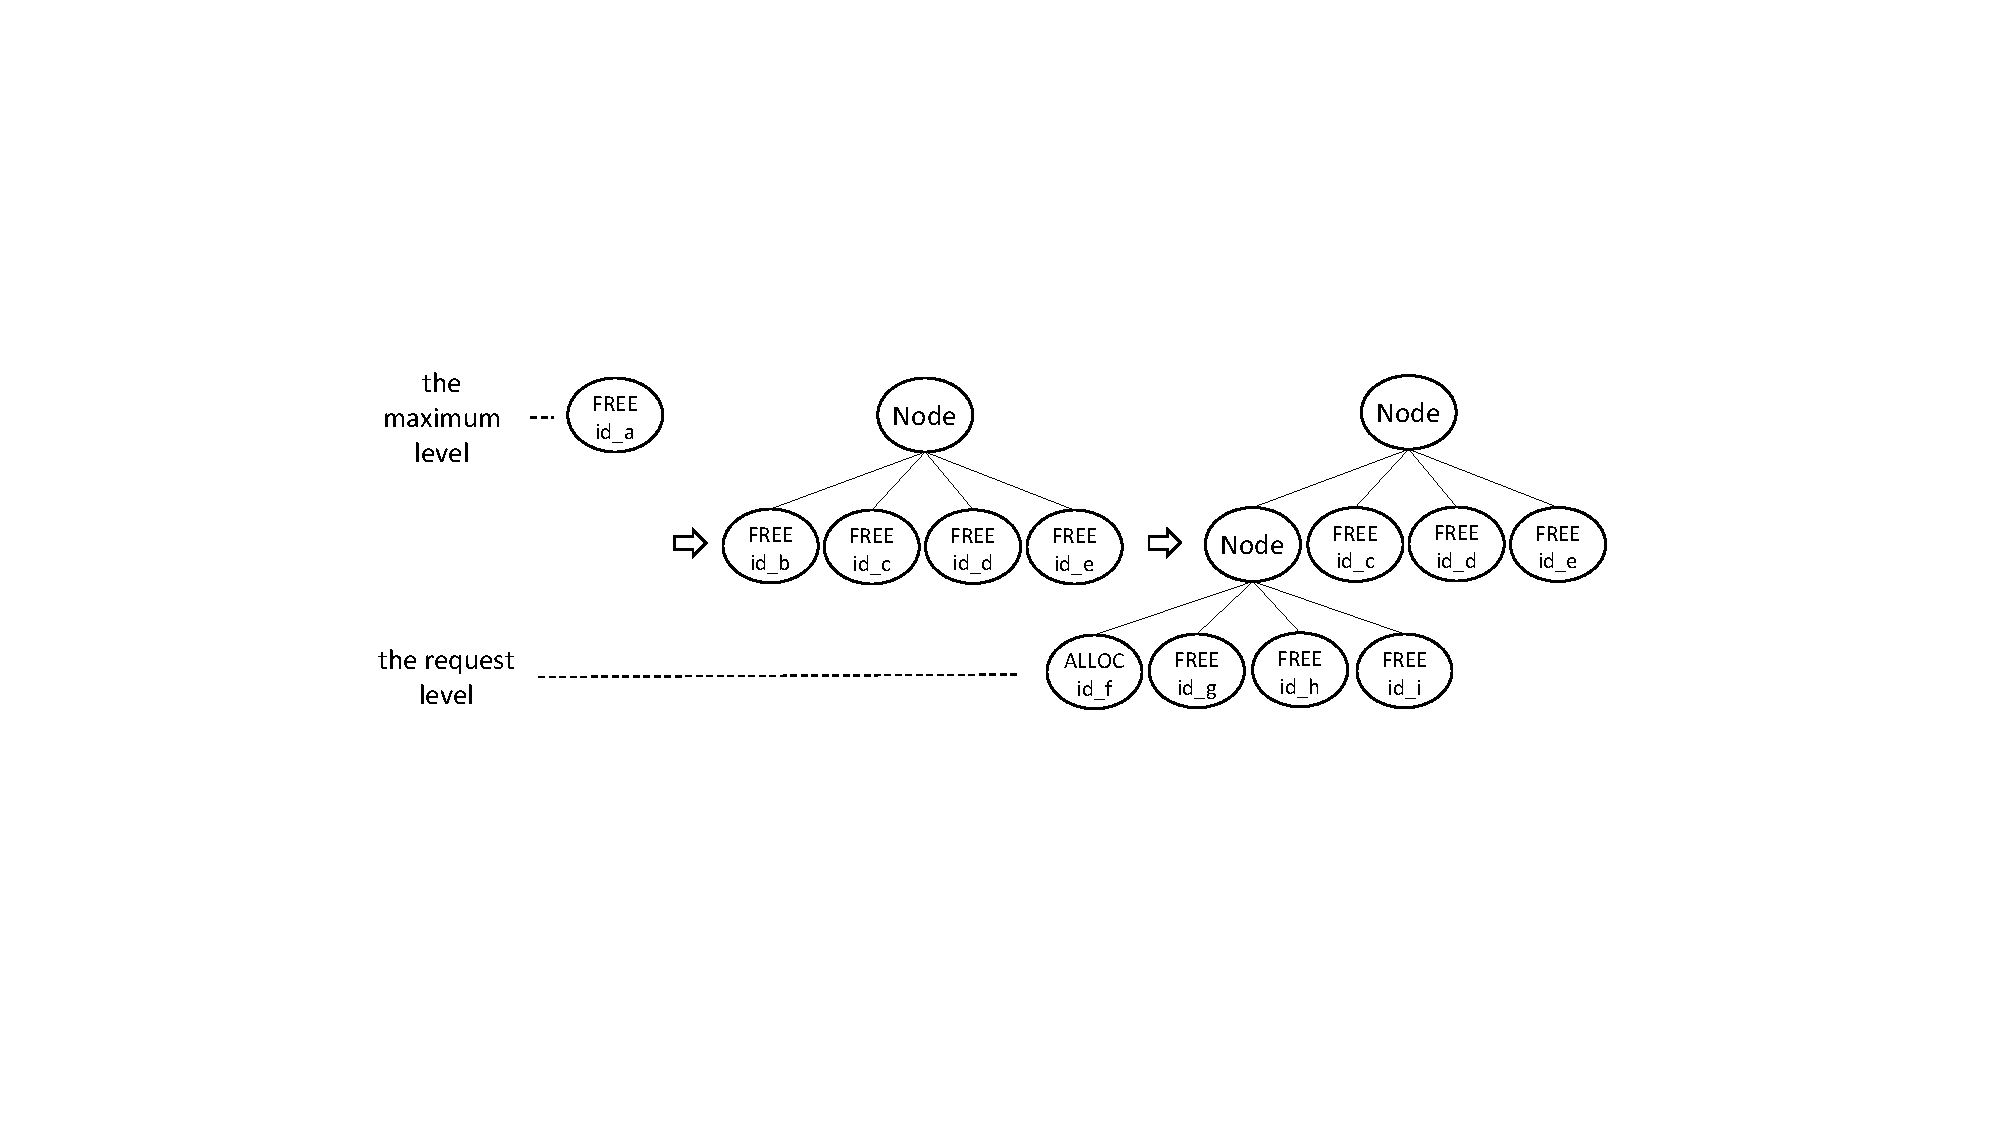
\includegraphics[width=1\textwidth]{fig1.pdf}
	\caption{The progress of dividing a free memory block}
	\label{fig1}
\end{figure}

\begin{definition} [Deallocation Operation] \\
	free blo\_set b $\equiv$ \\
	\phantom{x} \hspace{10pt} if $\exists$btree $\in$ blo\_set. b $\in$ tree.set btree then \\
	\phantom{x} \hspace{20pt} if type b = FREE then False \\
	\phantom{x} \hspace{20pt} else btree = THE t. t $\in$ blo\_set $\wedge$ b $\in$ tree.set t \\
	\phantom{x} \hspace{40pt} merge (reset btree b FREE) \\
	\phantom{x} \hspace{10pt} else False
\end{definition}

The deallocation progress firstly checks whether there is a quad-tree in \emph{blo\_set} that the occupied memory block to be released belongs to this tree. If there is no such tree, the procedure returns \emph{False}. Next, if the type of the occupied memory block is \emph{FREE}, the progress also returns \emph{False}. When all conditions are met, the memory block is returned to the tree it belongs to, thereafter merging operation is executed. The merging operation is to combine all free memory blocks that belong to the same parent tree showed in Fig. \ref{fig2}.

\begin{figure}
	\centering
	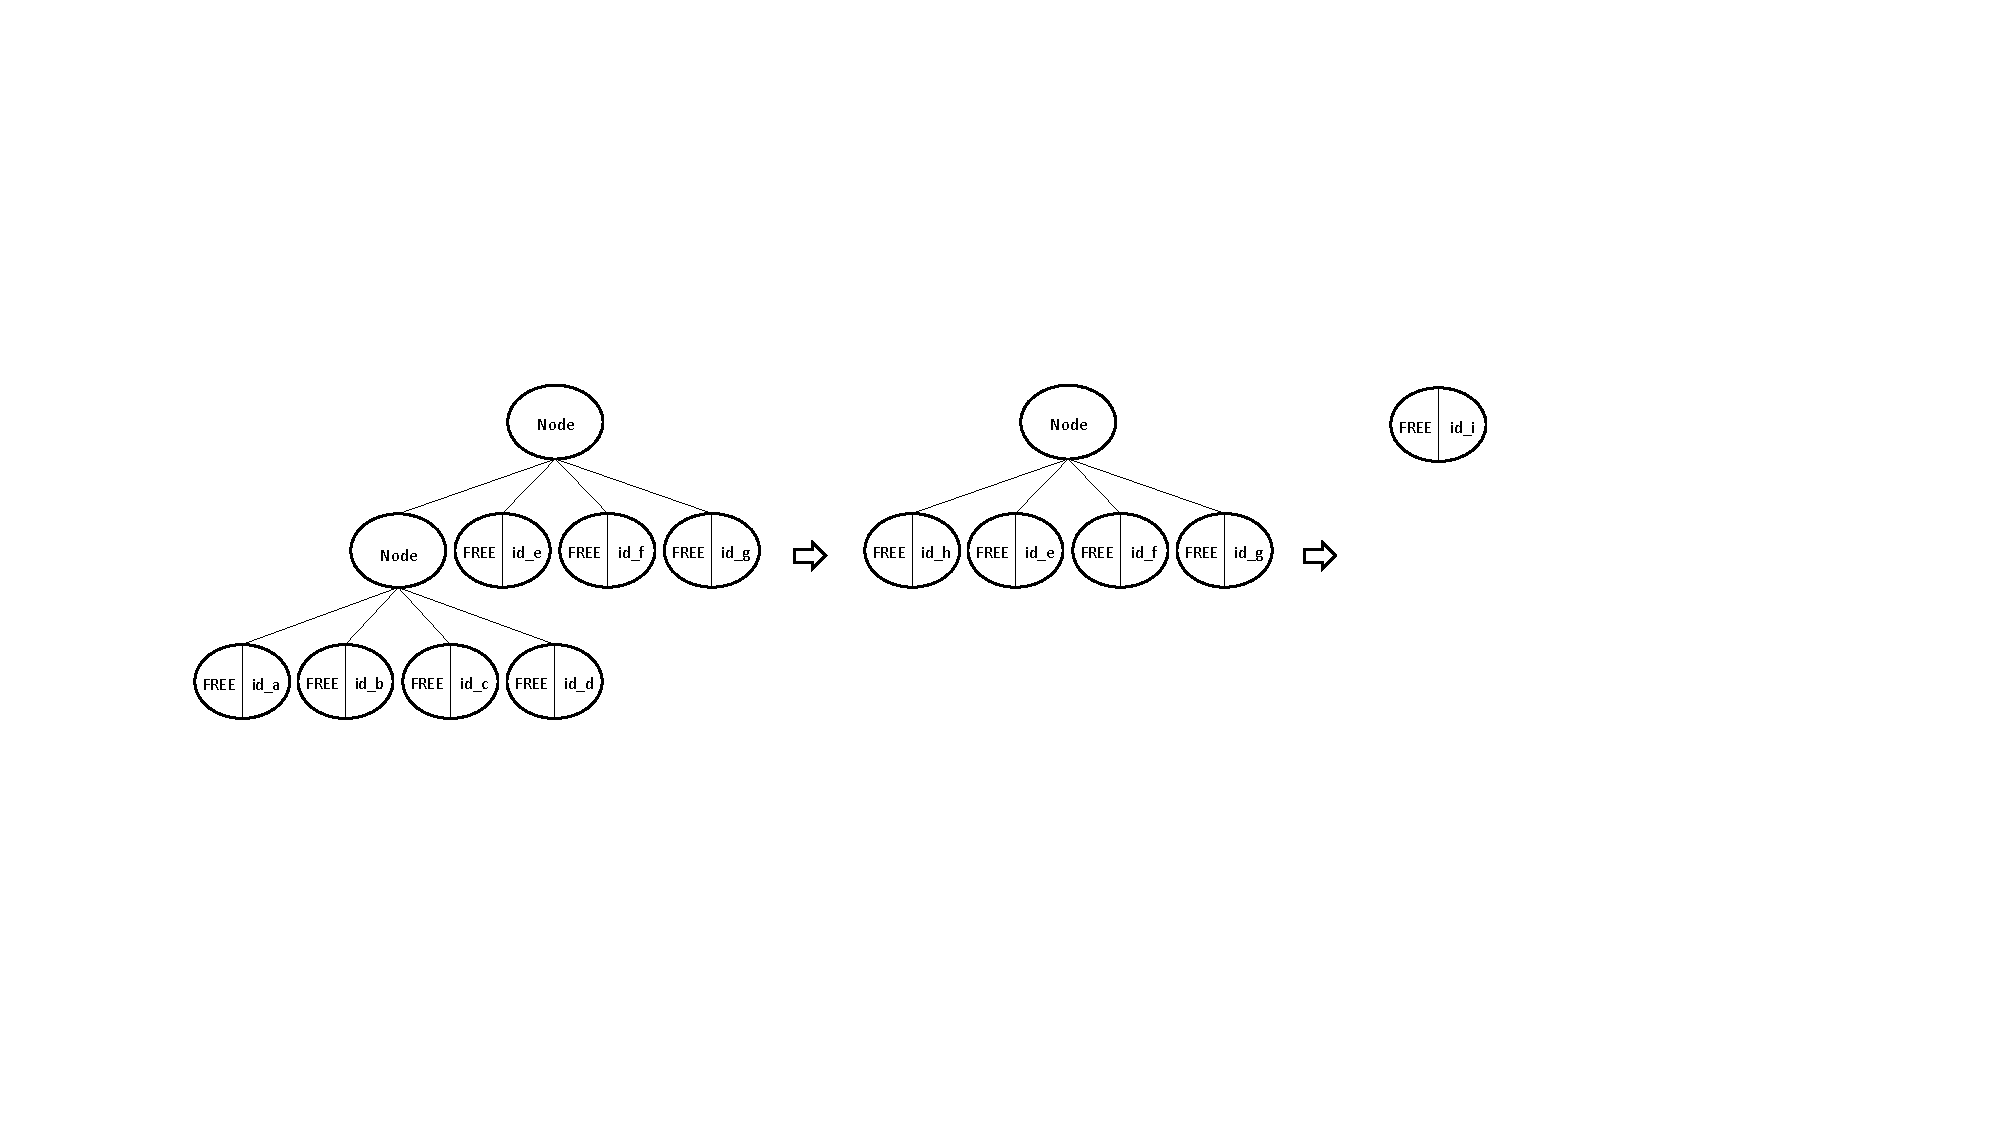
\includegraphics[width=1\textwidth]{fig2.pdf}
	\caption{The progress of merging all free memory blocks}
	\label{fig2}
\end{figure}

Owing to space constraints, the \emph{split} and the \emph{merge} operations constructed by induction are not described in detail. At this point, we have done the specification for the buddy memory algorithms. Next, we are going to verify the properties to guarantee the functional correctness of this specification.
